% IEEE Transactions-style research proposal (English)
% Compile: latexmk -pdf -interaction=nonstopmode main.tex
% IEEEtran provides the IEEE journal typography and two-column layout.
\documentclass[journal,10pt]{IEEEtran}
\usepackage[T1]{fontenc}
\usepackage{newtxtext,newtxmath}
\usepackage{graphicx}
\usepackage{booktabs}
\usepackage{tabularx}
\usepackage{array}
\usepackage{amsmath}
\usepackage{algorithm}
\usepackage{algpseudocode}
\usepackage{cite}
\usepackage{xurl}
\usepackage[hidelinks]{hyperref}
\urlstyle{same}
\newcommand{\egnea}{EG-NEA}
\begin{document}
\title{An Evidence-Grounded AI Agent for Natural-Language Nutrition and Exercise Tracking: A Verifiable System Design}
\author{Author Name, Student ID (to be completed)%
\thanks{Research proposal. Department and university affiliation to be completed by the authors.}}
\markboth{Research Proposal, November 2026}{Evidence-Grounded Nutrition and Exercise Agent}
\maketitle
\begin{abstract}
Obesity and unhealthy dietary behaviors have become major public health concerns worldwide. According to the World Health Organization, approximately 45\% of adults worldwide were overweight in 2024, including 940 million individuals living with obesity. In Taiwan, more than half of the adult population is classified as overweight or obese, highlighting the need for accessible and effective dietary monitoring systems. However, conventional calorie-tracking applications rely heavily on manual food searches, portion selection, and nutritional data entry, resulting in substantial cognitive and operational burdens. These limitations are particularly pronounced in Taiwanese dietary contexts, where colloquial food descriptions frequently involve mixed dishes, variable portion sizes, cooking methods, condiments, and restaurant-specific preparations.

To address these challenges, this study proposes DietSense, an explainable and culturally adapted dietary assessment agent that integrates natural language understanding, interactive clarification, retrieval-augmented generation (RAG), and deterministic nutritional computation. The proposed framework transforms free-form Traditional Chinese dietary descriptions into structured food records by identifying food categories, portion sizes, preparation methods, ingredients, and consumption-related attributes. An uncertainty-aware clarification mechanism dynamically generates targeted questions when essential information is missing or ambiguous, thereby reducing unsupported assumptions and potential errors associated with large language models. Furthermore, a retrieval-based nutritional grounding module incorporates authoritative food composition databases, including the Taiwan Food and Drug Administration and USDA FoodData Central, while a deterministic computation engine independently calculates energy intake and nutritional values to enhance transparency, traceability, and reproducibility.

A primary contribution of this study is the development of a benchmark dataset comprising 500 Taiwanese dietary descriptions covering local dishes, street foods, lunchboxes, beverages, and home-cooked meals. Each entry is designed to associate colloquial expressions with ingredient composition, portion information, preparation methods, and reference nutritional values. The proposed system will be evaluated using this benchmark, targeting at least 85\% of calorie estimates within $\pm$20\% of their reference values. In addition, a seven-day usability study involving 20 participants will investigate whether DietSense can reduce dietary logging time by approximately 60\% compared with conventional manual tracking while achieving a System Usability Scale score of at least 70.

By separating semantic interpretation from numerical nutritional computation, DietSense aims to establish a transparent, auditable, and culturally contextualized framework for AI-assisted dietary assessment. The proposed approach has potential applications in personalized dietary management, chronic disease prevention, clinical nutrition support, and public health research.
\end{abstract}
\begin{IEEEkeywords}
Dietary assessment, natural language processing, large language models, retrieval-augmented generation, nutritional estimation, explainable artificial intelligence, human--AI interaction, Taiwanese cuisine.
\end{IEEEkeywords}
\section{Introduction}
\subsection{Motivation and Background}
Dietary and exercise monitoring is relevant to public health and everyday self-management. WHO estimates indicate that overweight and obesity affect a substantial proportion of the adult population \cite{who}. Although food logs and activity trackers are widely available, recording every item manually requires time and nutrition knowledge. For example, a user may write, ``I ate a bowl of braised pork rice and drank 300 mL of soy milk, then jogged for half an hour.'' Such descriptions contain multiple events and often leave serving sizes, preparation methods, and activity intensities unspecified.

This proposal targets general adult self-monitoring in Traditional Chinese. The anticipated implementation uses a Python/Streamlit interface, a local SQLite database, an interchangeable GPT/Gemini language-model adapter, and food composition and activity-energy references.
\subsection{Problem Definition and Existing Limitations}
An LLM can interpret informal language, but its numerical answers are not inherently measured or verifiable. Food names may not map cleanly to nutrient tables, especially for regional dishes, and portion errors can dominate nutritional errors \cite{lemay,nutrients,imageeval,diabot}. Exercise-energy estimates based on metabolic equivalents (METs) represent approximate population-level values, not personalized calorimetry \cite{compendium}. Finally, a conversational assistant may make silent assumptions or modify a historical record without a reliable audit trail.

Existing community automations demonstrate the feasibility of connecting messaging interfaces, LLMs, and spreadsheets \cite{n8none,n8ntwo}, but those templates do not by themselves establish a validated nutrition-analysis method, uncertainty policy, or scientifically assessed error rate.
\subsection{Proposed Innovation and Contributions}
The proposed contribution is an integrated, testable workflow rather than a claim that individual components are novel: (1) a multi-intent Traditional Chinese event schema; (2) traceable food and exercise retrieval with explicit uncertainty and user confirmation; (3) deterministic energy accounting that avoids double-counting exercise expenditure; (4) an evidence-gated daily-report generator; and (5) reproducible baseline comparisons and model-agnostic Python components.

\section{Related Work}
The review deliberately covers both AI technology (language extraction, semantic food matching, agent workflows) and domain expertise (nutrition reference data, resting energy expenditure, METs, and measurement uncertainty).
\subsection{Literature and Technology Comparison}
Table~\ref{tab:related} compares representative scientific works and technical resources. The listed evidence types should not be treated as equivalent: peer-reviewed publications, official datasets, and community workflow templates serve different purposes.
\begin{table*}[!t]
\caption{Selected Related Work and Domain Resources (Proposal-Stage Synthesis)}
\label{tab:related}
\centering
\footnotesize
\setlength{\tabcolsep}{3.2pt}
\renewcommand{\arraystretch}{1.16}
\begin{tabularx}{\textwidth}{@{}p{0.45cm}p{0.65cm}XXXXXX@{}}
\toprule
Ref. & Year & Problem & AI method & Domain knowledge & Data / resource & Reported observation & Limitation\\
\midrule
\cite{lemay} & 2026 & Food-to-database matching & Semantic retrieval and LLM reranking & Food composition mapping & Dietary reference databases & Hybrid matching is promising & Coverage and no-match cases\\
\cite{nutrients} & 2026 & Text-based nutrient estimates & Comparative LLM assessment & Macro- and micronutrients & Common food descriptions & Performance varies by nutrient and prompt & Mixed dishes and uncertain quantities\\
\cite{imageeval} & 2025 & Image-based nutrition estimates & Multimodal LLMs & Portions and nutrient estimation & Standardized food images & Feasible but error-prone estimates & Portion and image variation\\
\cite{diabot} & 2025 & Dietary assessment in Taiwan & Customized multimodal chatbot & Local diet assessment & Taiwanese dietary images & Domain customization is relevant & Portion and generalization challenges\\
\cite{foody} & 2026 & Food-domain language models & Specialized food LLM & Food ontologies and nutrition & Domain QA resources & Domain adaptation offers opportunities & Domain data and transferability\\
\cite{compendium} & 2024 & Activity-energy reference & Not AI; MET compilation & Exercise physiology & Adult Compendium & Reference values across activities & Group estimates, not individual measurements\\
\cite{mifflin} & 1990 & Resting energy expenditure & Predictive regression & Metabolism and anthropometry & Adult participants & Widely used REE equation & Individual prediction error\\
\bottomrule
\end{tabularx}
\end{table*}

\subsection{Research Gap}
The reviewed literature suggests four interacting challenges: ambiguous natural language, imperfect food-reference matching, uncertain serving sizes and activity intensities, and insufficiently traceable generated recommendations. The project therefore investigates whether a unified pipeline---structured extraction, retrieval, deterministic calculation, provenance, and selective human confirmation---improves reliability over a direct LLM response. This is a \emph{research hypothesis}, not a demonstrated superiority claim.

\section{Deep Research: Domain Reasoning}
\subsection{Five Core Mental Models}
\textbf{1) Separate observation from estimation.} Portion sizes, activity METs, and resting energy expenditure may be estimated rather than measured \cite{imageeval,compendium,mifflin}. Therefore, numeric fields carry their sources, estimate flags, and uncertainty metadata.

\textbf{2) Prefer evidence chains to plausible outputs.} An interpreted food item must be associated with a food-composition record, preparation state, and source/version, where available \cite{lemay,usda}. This enables reproducible calculations and meaningful corrections.

\textbf{3) Account for compounded uncertainty.} Energy is the product of quantity and energy density, so errors in either contribute to the result. Portion uncertainty is explicitly displayed rather than hidden by precise decimal formatting \cite{nutrients,imageeval}.

\textbf{4) Separate total from incremental activity energy.} MET-derived gross expenditure includes resting energy, while activity factors may already incorporate exercise \cite{compendium,mifflin}. The system uses a documented baseline policy and prevents repeated addition of the same activity.

\textbf{5) Favor longitudinal, non-diagnostic feedback.} A single day's calorie difference does not establish a health diagnosis. Accordingly, the reporting agent emphasizes trends, data completeness, and appropriately bounded suggestions rather than clinical prescriptions \cite{who}.

\subsection{Three Major Debates}
\textbf{Debate 1---LLM-only estimates versus database-grounded calculations.} Direct generation minimizes system complexity, whereas retrieval improves auditability. Existing assessment work raises concerns about variable nutrition estimates, while food matching studies motivate retrieval-assisted strategies \cite{nutrients,lemay}. The project adopts database-based arithmetic and tests whether the additional steps yield a measurable benefit. Unresolved issue: limited coverage of regional mixed dishes.

\textbf{Debate 2---Frictionless automation versus human confirmation.} Automatic logging reduces user effort, but unknown portions and ambiguous changes can produce persistent errors. Studies of dietary estimation motivate caution \cite{imageeval,diabot}. The proposed compromise is risk-based clarification; whether prompts reduce long-term usability remains to be tested.

\textbf{Debate 3---Population equations versus personalized expenditure.} Standard REE formulas and MET tables are low-cost and transparent, while wearable or measured data may better reflect individual conditions but introduce device error, access constraints, and privacy considerations \cite{mifflin,compendium}. The first version uses transparent estimates and permits future calibration.

\subsection{Ten Questions for Deep Understanding}
\begin{enumerate}
\item \emph{Why} does schema-valid JSON not imply a correct calorie estimate? Because extraction format does not validate food identity, quantity, or reference data.
\item \emph{What if} a meal is described only as ``one lunch box''? Decompose where possible; request missing details or display an explicit range.
\item \emph{What trade-off} arises when the LLM directly returns calories? Simplicity is gained at the cost of provenance and repeatability.
\item \emph{What failure case} occurs when one utterance both adds and deletes entries? Conflicting intents require exact record identifiers and transactional confirmation.
\item \emph{What evidence} would favor the hybrid system? Held-out cases with lower energy error and unsafe-write rate at acceptable latency and cost.
\item \emph{How do} gross and net MET expenditure differ? Gross includes the resting-energy component, which can overlap a daily baseline.
\item \emph{When should} an API be called rather than a local function? Language ambiguity may require an LLM; deterministic arithmetic does not.
\item \emph{How should} ``yesterday I jogged'' be interpreted? Resolve relative dates against a recorded local timezone and request clarification if necessary.
\item \emph{Why preserve} historical nutrient snapshots? Reference-database updates must not silently rewrite past calculations.
\item \emph{What if} a generated report contradicts verified records? Remove or regenerate unsupported claims using an evidence gate.
\end{enumerate}

\section{Proposed Scheme}
\subsection{Application Scenario}
A user enters informal Traditional Chinese text covering meals, activity, dates, or changes to earlier records. The system identifies the requested operations, retrieves evidence, computes values, presents ambiguous items for review, and saves confirmed events. It can subsequently produce a daily or multi-day report without diagnosing disease or prescribing treatment.
\subsection{System Architecture}
The 11 numbered modules in Fig.~\ref{fig:architecture} are: \textbf{(1)} Streamlit interaction; \textbf{(2)} planner and intent agent; \textbf{(3)} schema validation (types, units, dates); \textbf{(4)} food retrieval (local and optional USDA); \textbf{(5)} MET activity retrieval; \textbf{(6)} historical log lookup; \textbf{(7)} deterministic Python analytics; \textbf{(8)} domain knowledge and safety rules; \textbf{(9)} evidence-constrained report agent; \textbf{(10)} human review and confirmation; and \textbf{(11)} SQLite storage, source provenance, and audit history.
\begin{figure}[!t]
\centering
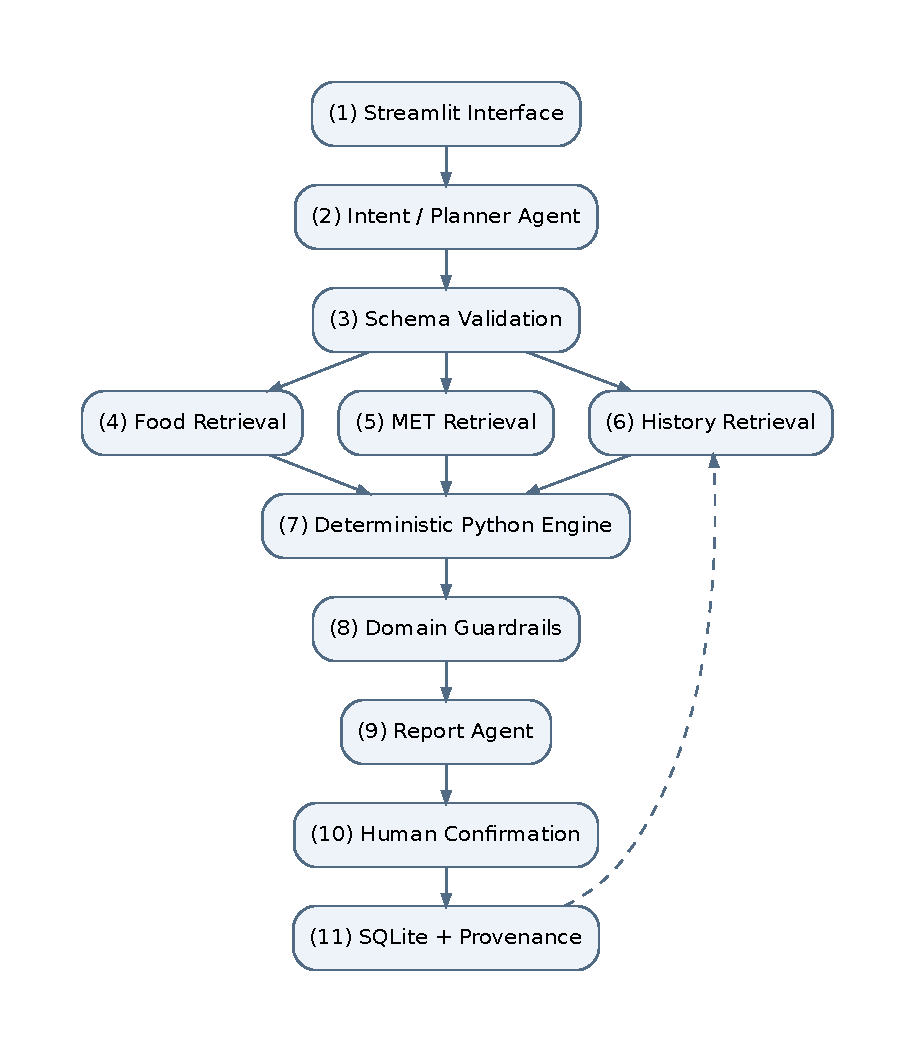
\includegraphics[width=\columnwidth]{figures/architecture.pdf}
\caption{Proposed evidence-grounded AI agent architecture with numbered modules.}
\label{fig:architecture}
\end{figure}
\subsection{Processing Flow and Exception Policy}
Fig.~\ref{fig:flowchart} shows input, intent parsing, schema inspection, retrieval, uncertainty decisions, deterministic analysis, confirmation, persistence, and report generation. A missing food match, ambiguous record identifier, unavailable API, or invalid unit must not cause a silent database update. Clarification or a transparent failure response is preferred.
\begin{figure}[!t]
\centering
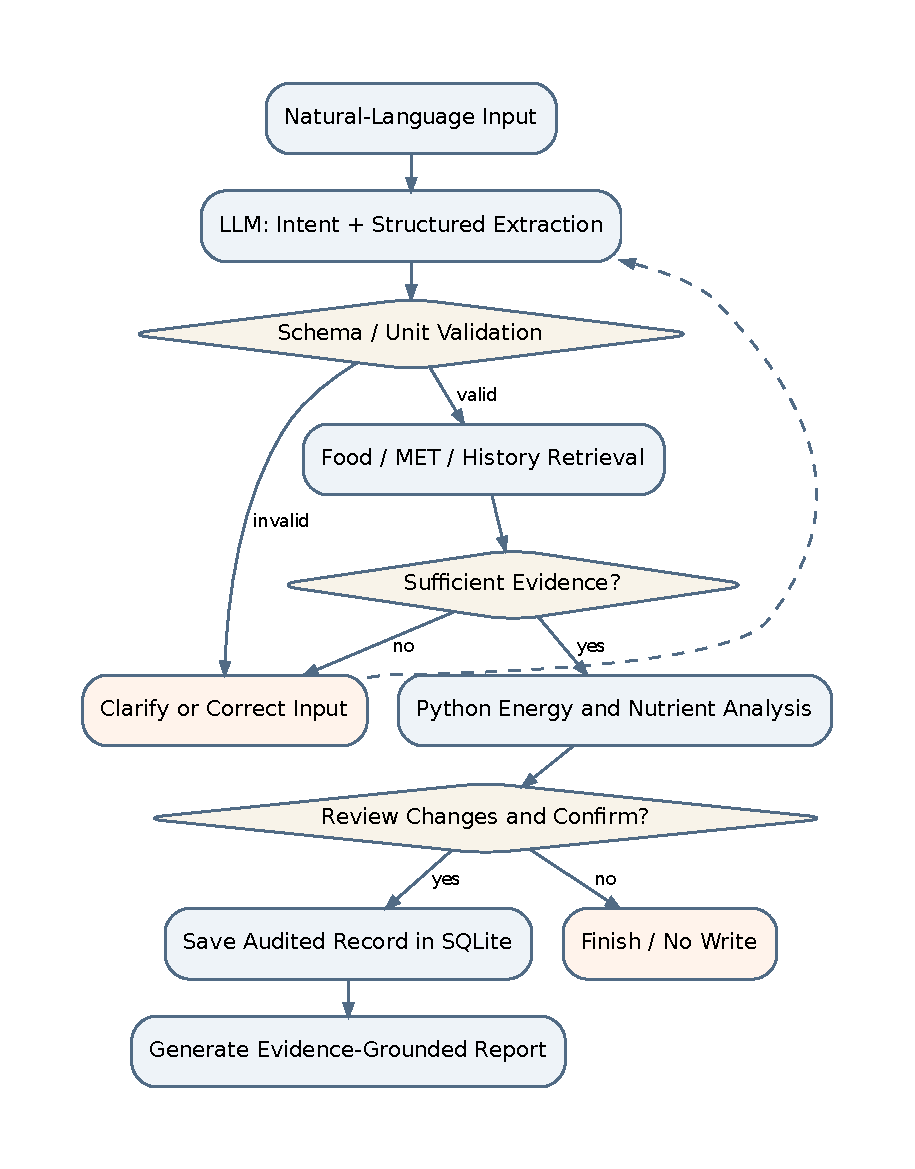
\includegraphics[width=\columnwidth]{figures/flowchart.pdf}
\caption{Input-to-report workflow with validation, clarification, and safe-update branches.}
\label{fig:flowchart}
\end{figure}
\subsection{Core Agent Algorithm}
\begin{figure}[!t]
\centering
\begin{minipage}{\columnwidth}
\small\textbf{Algorithm 1: Evidence-Grounded Nutrition and Exercise Agent}
\vspace{3pt}\hrule\vspace{3pt}
\begingroup\ttfamily\fontsize{7.5}{9.3}\selectfont
\noindent Input: query Q, profile U, history H, food DB F, MET DB M\\
Output: confirmed records and report R\\
01 parse intent, slots, ambiguity from Q\\
02 if schema invalid: request clarification\\
03 if intent includes FOOD:\\
04 \quad candidates = retrieve(F, food names, top-k)\\
05 \quad choices = rerank(candidates, context)\\
06 \quad if no match or unknown portion: clarify\\
07 \quad compute nutrients from verified grams\\
08 if intent includes EXERCISE:\\
09 \quad activity = lookup(M, type, intensity)\\
10 \quad if intensity absent: mark uncertain\\
11 \quad gross = MET*3.5*kg*min/200\\
12 \quad net = max(0,MET-1)*3.5*kg*min/200\\
13 if REPORT: retrieve dated history\\
14 if UPDATE/DELETE: resolve exact entry ID\\
15 validate all numerical computations\\
16 preview changes; require confirmation\\
17 if confirmed: store data and provenance\\
18 compute REE, TDEE and daily summaries\\
19 run domain and uncertainty checks\\
20 generate evidence-grounded explanation R\\
21 remove or regenerate unsupported claims\\
22 return records, summaries, warnings, R
\endgroup
\vspace{3pt}\hrule
\end{minipage}
\end{figure}
\subsection{Domain Formulas and Data Modeling}
The Mifflin--St Jeor predictive equations for resting energy expenditure (REE) use mass $w$ in kilograms, height $h$ in centimeters, and age $a$ in years \cite{mifflin}:
\begin{equation}
\widehat{\mathrm{REE}}=10w+6.25h-5a+\begin{cases}+5,&\text{male equation},\\-161,&\text{female equation}.\end{cases}
\label{eq:ree}
\end{equation}
A simple total daily energy expenditure estimate is $\widehat{\mathrm{TDEE}}=\widehat{\mathrm{REE}}\times A$, where the activity factor $A$ must be defined consistently with any logged activity. Food energy is evaluated as
\begin{equation}
E_{\mathrm{food}}=\sum_{i=1}^{n}\frac{m_i}{100}\,\rho_i,
\label{eq:food}
\end{equation}
where $m_i$ is food mass in grams and $\rho_i$ is reference kilocalories per 100 g. For activity duration $t$ (minutes) and MET value $M$:
\begin{align}
E_{\mathrm{gross}}&\approx M\frac{3.5w}{200}\,t,\\
E_{\mathrm{net}}&\approx\max(0,M-1)\frac{3.5w}{200}\,t.
\label{eq:met}
\end{align}
The net estimate is only added to a baseline that excludes the corresponding activity; a daily activity multiplier that already includes a workout must not double-count it. The database design includes \texttt{users}, \texttt{foods}, \texttt{activity\_mets}, \texttt{entries}, \texttt{food\_log\_items}, \texttt{exercise\_log\_items}, \texttt{agent\_runs}, and \texttt{reports}. Records retain original text, normalized fields, reference versions, estimated/confirmed flags, and audit history.

\section{Evaluation Plan}
\subsection{Data and Case Studies}
The planned test set contains at least 150 Traditional Chinese utterances (single foods, Taiwanese mixed dishes, missing portions, combined food/exercise, relative dates, and revisions), 50 manually checked food-matching cases, 30 activity-energy cases, and 20 edit/clarification cases. Where feasible, at least 10 consenting adult volunteers will undertake representative tasks. Researcher-authored evaluation utterances will be explicitly distinguished from real-world user-collected data; two annotators will review reference labels.
\subsection{Baselines and Metrics}
\textbf{B1:} direct LLM calorie response; \textbf{B2:} keyword/rule extraction followed by lookup; \textbf{Proposed:} structured LLM extraction with top-$k$ retrieval, verified arithmetic, and human confirmation. Metrics include intent accuracy, micro-F1 for extracted slots, top-1/top-5 food matching, no-match recall, energy mean absolute error (MAE), carefully conditioned mean absolute percentage error (MAPE), activity estimation error, unsafe-write rate, clarification rate, median and 95th-percentile latency, API cost per 100 records, and user task completion time. Very small reference energy values are excluded or handled separately for MAPE.
\subsection{Ablation and Reproducibility}
Ablations remove retrieval, confirmation, or domain safeguards; GPT- and Gemini-based parsers are compared under matched schemas. Evaluation cases will be separated by dish or author where possible to prevent template leakage. Prompt versions, model identifiers, decoding parameters, reference-data versions, and API timestamps will be recorded. \emph{All experimental outcomes remain pending.}

\section{Risks, Ethics, and Limitations}
The proposed tool is intended for general adult self-monitoring and not for medical diagnosis, individualized treatment, or high-risk dietary prescriptions. API calls will minimize personally identifiable and sensitive data; local historical records must be deletable, and access credentials must be excluded from source control. When data sources or quantities are insufficient, the system reports an estimate or requests clarification rather than fabricating precise figures. Accuracy, user burden, and external validity require empirical evaluation.

\section{Expected Contributions and Conclusion}
The expected outcomes are: (i) an auditable natural-language nutrition/activity logging pipeline; (ii) repeatable, source-linked energy calculations; (iii) safer correction and confirmation mechanisms; and (iv) a transparent benchmark for evaluating accuracy, interaction cost, and latency. These outcomes are research goals, not established findings. The project will test whether combining language understanding with domain-grounded retrieval and deterministic computation offers a practical reliability advantage over direct AI-generated estimates.

\begin{thebibliography}{99}
\bibitem{who} World Health Organization, ``Obesity and overweight,'' fact sheet. [Online]. Available: \url{https://www.who.int/news-room/fact-sheets/detail/obesity-and-overweight}
\bibitem{lemay} Lemay \emph{et al.}, ``Evaluation of large language models for mapping dietary data to food databases,'' \emph{The Journal of Nutrition}, 2026, doi: 10.1016/j.tjnut.2026.101678.
\bibitem{nutrients} ``Evaluation of energy and nutrient estimates from large language models using text-based queries,'' \emph{The Journal of Nutrition}, 2026, doi: 10.1016/j.tjnut.2026.101712.
\bibitem{imageeval} ``Performance evaluation of 3 large language models for nutritional content estimation from food images,'' \emph{Current Developments in Nutrition}, 2025, doi: 10.1016/j.cdnut.2025.107556.
\bibitem{diabot} ``Customized multimodal Diabot-GPT-4o enhances accuracy of image-based dietary assessments in dietetic trainees in Taiwan,'' 2025. [Online]. Available: \url{https://pubmed.ncbi.nlm.nih.gov/41138916/}
\bibitem{foody} ``Large language models in food and nutrition science: Opportunities, challenges, and the case of FoodyLLM,'' \emph{Current Research in Food Science}, 2026, doi: 10.1016/j.crfs.2026.101351.
\bibitem{compendium} S. D. Herrmann \emph{et al.}, ``2024 Adult Compendium of Physical Activities: A third update of the energy costs of human activities,'' \emph{J. Sport Health Sci.}, 2024. [Online]. Available: \url{https://pmc.ncbi.nlm.nih.gov/articles/PMC10818145/}
\bibitem{mifflin} M. D. Mifflin \emph{et al.}, ``A new predictive equation for resting energy expenditure in healthy individuals,'' \emph{Am. J. Clin. Nutr.}, vol. 51, no. 2, pp. 241--247, 1990, doi: 10.1093/ajcn/51.2.241.
\bibitem{usda} U.S. Department of Agriculture, ``FoodData Central API guide.'' [Online]. Available: \url{https://fdc.nal.usda.gov/api-guide/}
\bibitem{openai} OpenAI, ``Structured outputs,'' API documentation. [Online]. Available: \url{https://developers.openai.com/api/docs/guides/structured-outputs}
\bibitem{gemini} Google, ``Structured output,'' Gemini API documentation. [Online]. Available: \url{https://ai.google.dev/gemini-api/docs/structured-output}
\bibitem{n8none} n8n Community, ``Nutrition tracker and meal logger with Telegram, Gemini AI and Google Sheets,'' workflow template no. 7756. [Online]. Available: \url{https://n8n.io/workflows/7756-nutrition-tracker-and-meal-logger-with-telegram-gemini-ai-and-google-sheets/}
\bibitem{n8ntwo} n8n Community, ``Track nutrition and fitness via webhook with OpenAI, Google Sheets and Slack alerts,'' workflow template no. 14858. [Online]. Available: \url{https://n8n.io/workflows/14858-track-nutrition-and-fitness-via-webhook-with-openai-google-sheets-and-slack-alerts/}
\end{thebibliography}
\end{document}
